\chapter{Zusammenfassung und Probleme}

\section{Zusammenfassung}
In diesem Projekt wurde ein Tool entwickelt, das es ermöglicht, Dreiecke eines
3D-Modells in Triangle Strips umzuwandeln und diese effizient zu rendern. Die
Implementierung basierte auf einem bestehenden Projekt und umfasste mehrere
zentrale Komponenten:

\begin{itemize}
    \item \textbf{Implementierung des Triangles-to-Strip Konverters:} \\
    Dieser Konverter wandelt Dreiecke in Triangle Strips um, um die Effizienz beim Rendern zu erhöhen.
    \\
    \item \textbf{Implementierung des Strip-Zeichners:} \\
    Der Zeichner rendert die Triangle Strips unter Verwendung von OpenGL.
    \\
    \item \textbf{Implementierung der Steuerung und der GUI:} \\
    Die Steuerung wurde angepasst und eine benutzerfreundliche Oberfläche wurde mithilfe von ImGui entwickelt, um Interaktionen mit dem Tool zu ermöglichen.
    \\
    \item \textbf{Weitere Anpassungen:} \\
    Verschiedene Code-Änderungen und Optimierungen wurden vorgenommen, um die neuen Funktionalitäten zu integrieren und die Performance zu verbessern. Dabei wurden auch die entsprechenden Header-Dateien angepasst.
\end{itemize}

\section{Probleme}
Während der Entwicklung traten einige Herausforderungen auf, insbesondere bei
der Integration und Optimierung der verschiedenen Komponenten. Ein spezifisches
Problem, das nicht vollständig behoben werden konnte, ist eine gelegentliche
Assertion beim Laden eines Meshes (siehe Abbildung \ref{fig:Error}). Dieser Fehler konnte bisher nicht
eindeutig reproduziert oder behoben werden. Dies deutet auf ein potenzielles
Problem in der Speicherverwaltung oder Indexierung hin, das weitere
Untersuchungen erfordert.

\begin{figure}[ht]
    \centering
    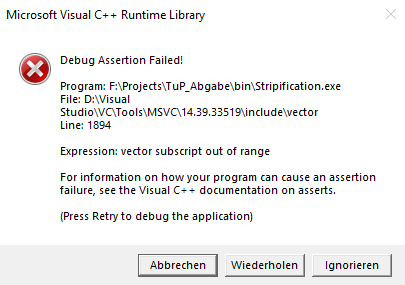
\includegraphics[scale = 0.75]{images/Error.PNG}
    \caption{Assertion - vector subscript out of range}
	\label{fig:Error}
\end{figure} 